\section{Classification}

\begin{frame}
    \frametitle{Classification}

    \begin{columns}
        \begin{column}{0.5\textwidth}
            Given data points \(\vec{x}_1, \vec{x}_2, \ldots, \vec{x}_m\) and labels \(\ell_1, \ell_2, \ldots, \ell_m\), and \(\ell_i = \pm 1\), we want to find a vector \(\vec{w}\) such that all points with label \(1\) have a positive inner product and all points with label \(-1\) have a negative inner product.
            We accomplish this by assigning a \emph{cost function} \(c(\vec{x}^T \vec{w}, \ell_i)\)and try to minimize this cost function.
            Least squares is one type of cost function, but we can define new ones.
        \end{column}
        \begin{column}{0.5\textwidth}
            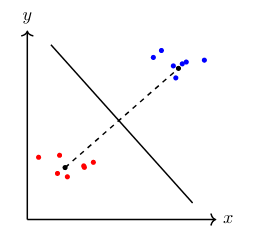
\includegraphics[width=\textwidth]{images/classification.png}
        \end{column}
    \end{columns}
\end{frame}

\begin{frame}
    \frametitle{Quadratic Approximation}

    We can linearize a quadratic cost function in the form
    \begin{align}
        c(\vec{w}^\ast + \vec{\delta w}) \approx c(\vec{w}^\ast) +
        \begin{bmatrix}
            \frac{\partial c}{\partial w_1} & \frac{\partial c}{\partial w_2} & \cdots & \frac{\partial c}{\partial w_n}
        \end{bmatrix} (\vec{\delta w}) \\
        + \frac{1}{2} (\vec{\delta w})^T
        \underbrace{\begin{bmatrix}
            \frac{\partial^2 c}{\partial w_1 \partial w_1} & \cdots & \frac{\partial^2 c}{\partial w_1 \partial w_n} \\
            \vdots & \ddots & \vdots \\
            \frac{\partial^2 c}{\partial w_n \partial w_1} & \cdots & \frac{\partial^2 c}{\partial w_n \partial w_n}
        \end{bmatrix}}_{\text{Hessian}} (\vec{\delta w})
    \end{align}
\end{frame}
